\documentclass{zjgsureport}


\major{数学与应用数学}
\name{ze}
% \title{matlab程序设计}
\stuid{12345678}
\college{统计与数学学院}
\task{文稿、代码、作图}
\date{\zhtoday}
\expname{期末大作业}%课程作业/报告的题目
\course{最优化及其应用}%课程名称
\teacher{崔峰}
\renewcommand{\abstractname}{\large 摘要\\}%重定义摘要二字的大小
\newcommand{\upcite}[1]{\textsuperscript{\textsuperscript{\cite{#1}}}}


\graphicspath{ {images/} }

%-----------------------------------------BEGIN DOC----------------------------------------
\begin{document}

\makecover  %生成封面

%-----------------------------------------ABSTRACT-------------------------------------
\begin{abstract}
请在这里输入摘要内容.
\end{abstract}
\newpage


%-----------------------------------------CONTENT-------------------------------------
\thispagestyle{empty}
\tableofcontents



%------------------------------------------TEXT--------------------------------------------
\newpage
\setcounter{page}{1}


\section{常用代码模板}


\subsection{公式} 

\begin{equation*}
    \frac{\partial r_i(x)}{\partial x_j}=
    \begin{cases} -1& j=i-1\\ 2+3h^2(x_i+t_i+1)^2/2& j=i\\ -1& j=i+1\\0& else \end{cases}
    ,\quad 1\leq i \leq m
\end{equation*}



\begin{equation*}
\frac{\partial(r_1(x),\cdots,r_n(x))}{\partial (x_1(x),\cdots,x_n(x))}=
\begin{bmatrix}
\frac{\partial r_1(x)}{\partial x_1} & -1 & 0 & 0& \cdots & 0& 0 \\
-1 & \frac{\partial r_2(x)}{\partial x_2} & -1& 0 & \cdots & 0 & 0\\
0& -1 & \frac{\partial r_3(x)}{\partial x_3} & -1  & \cdots& 0& 0 \\
\vdots & \vdots & \vdots & \vdots & \ddots& \vdots& \vdots \\
0 & 0 &0 & 0 & \cdots & \frac{\partial r_{m-1}(x)}{\partial x_{n-1}}& -1\\
0 & 0 &0 & 0 & \cdots & -1 &\frac{\partial r_m(x)}{\partial x_n}\\
\end{bmatrix}
\end{equation*}


\begin{equation*}
    \nabla f(x)_j=
    2((\frac{\partial r_j(x)}{\partial x_j})r_j(x)-r_{j-1}(x)-r_{j+1}(x))
    ,\quad 1\leq j \leq n,r_0(x)=r_{n+1}(x)=0
\end{equation*}

\begin{equation*}
\begin{aligned}
\nabla f(x)_1&=2 \sum\limits_{i=1}^m (\frac{\partial r_i(x)}{\partial x_j})r_i(x)\\
&=2 \sum\limits_{i=1}^{29} (\frac{\partial r_i(x)}{\partial x_1})r_i(x)+2(\frac{\partial r_{30}(x)}{\partial x_1})r_{30}(x)+2(\frac{\partial r_{31}(x)}{\partial x_1})r_{31}(x)\\
&=2 \sum\limits_{i=1}^{29} (\frac{\partial r_i(x)}{\partial x_1})r_i(x)+2x_1-4x_1(x_2-x_1^2-1)\\
\end{aligned}
\end{equation*}


\newpage

\subsection{表格} 

\begin{table}[htp]
\caption{使用FR法解决二次型问题}\label{tab:FRCG}
\begin{center}
	\begin{tabular}{l|l}
	\hline
	1 &$k\leftarrow0,g_1\leftarrow\nabla f(x^{(1)}),d^{(1)}\leftarrow-g_1$\\ 
	2 &if $||\nabla f(x^{(1)})||\leq gtol$:\\ 
	3 &\quad return $x^{(1)}$ \\ 
	4 &while k $\leq$ MaxIter:\\ 
	5 &\quad $\lambda_k\leftarrow\dfrac{-g_k^T d^{(k)}}{d^{(k)T}Ad^{(k)}}$ \\
	6 &\quad $x^{(k+1)}\leftarrow x^{(k)}+\lambda_k d_{(k)}$ \\ 
	7 &\quad if $||\nabla f(x^{(k)})||\leq gtol$: \\ 
	8 &\quad \quad return $x^{(k)}$ \\ 
	9 &\quad $\beta_k\leftarrow\dfrac{||g_{k+1}||^2}{||g_k||^2}$ \\
	10 &\quad $d^{(k+1)}\leftarrow-g_{k+1}+\beta_kd^{(k)}$ \\ 
	11 &\quad $k\leftarrow k+1$ \\ 
	12 &return $x^{(k)}$\\ \hline
	\end{tabular}
\end{center}
\end{table}

表格引用:表\ref{tab:FRCG}.



\subsection{图片} 

\begin{figure}[!htp]
 \centering
 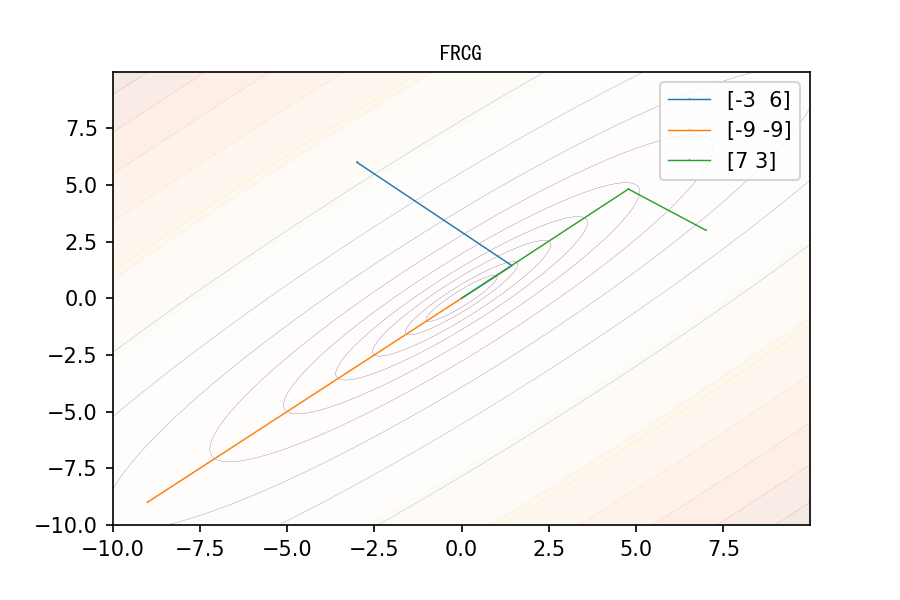
\includegraphics[height=7cm]{images/FRCG.png}
 \caption{用于正定二次函数的共轭梯度法}
 \label{fig:FRCG}
\end{figure}

图片引用:图\ref{fig:FRCG}.



\subsection{其他} \label{else}

章节引用:节\ref{else}。

文献引用:\cite{Erdos01}或\upcite{Erdos01}。

使用FR法解决二次型问题的Python代码参见附录\ref{sub:FRCG}.




% -----------------------------------REFERENCE----------------------------------------
\newpage
\begin{thebibliography}{99}
    \bibitem{Erdos01}Jorge J. Moré, Burton S. Garbow, and Kenneth E. Hillstrom. 1981. Testing Unconstrained Optimization Software. ACM Trans. Math. Softw. 7, 1 (March 1981), 17–41. 
\end{thebibliography}




% -----------------------------------Appendix----------------------------------------
\appendix
\newpage
\section{附录一:matlab代码}

\begin{lstlisting}[language=matlab]
[X, Y] = meshgrid(0.01:0.01:1, 0.01:0.01:1); 
Zfun =@(x,y)12.5*x.*log10(x).*y.*(y-1)+exp(-((25 ... 
*x - 25/exp(1)).^2+(25*y-25/2).^2).^3)./25; 
Z = Zfun(X,Y); 
figure; 
surf(Y,Z,X,'FaceColor',[1 0.75 0.65],'linestyle','none'); 
hold on 
surf(Y+0.98,Z,X,'FaceColor',[1 0.75 0.65],'linestyle','none'); 
axis equal; 
view([116 30]); 
camlight; 
lighting phong; % 设置光照和光照模式
\end{lstlisting}

\section{附录二:python代码}\label{sub:FRCG}
使用FR法解决二次型问题的Python代码如下:
\begin{lstlisting}[language=python]
def FRCG(x,grad,A,gtol=1e-6,maxit=200):
    out = dict()
    out['x']=[x]
    g = grad(x)
    nrmg = np.linalg.norm(g, ord=2)
    if nrmg<=gtol:
        out['iter']=[0]
        return out
    d=-g
    for iter in range(1, maxit + 1):
        out['iter']=iter
        lam=-np.dot(g.T,d)/np.dot(d.T,np.dot(A,d))
        x=x+lam*d
        out['x']+=[x]
        gp=g
        g = grad(x)
        nrmg = np.linalg.norm(g, ord=2)
        if nrmg<=gtol:
            break
        beta=np.dot(g.T,g)/np.dot(gp.T,gp)
        d=-g+beta*d
    return out
def grad(x):
    return np.array([0.52*x[0]-0.48*x[1], -0.48*x[0]+0.52*x[1]])
A=np.array([[0.52,-0.48],[-0.48,0.52]])
out=FRCG(np.array([3,4]),grad,A)
\end{lstlisting}


\end{document}
